\documentclass[border=3pt, tikz]{standalone}

\usepackage{tikz}
\usepackage{amsmath}
\usepackage{nccmath}
\usepackage{pgfplots}

\pgfplotsset{compat=1.17}

\usepackage{xcolor}
\colorlet{myred}{red!80!black}
\colorlet{myblue}{blue!80!black}
\colorlet{mybluee}{myblue!80!black}
\colorlet{mygreen}{green!60!black}
\colorlet{myorange}{orange!70!red!60!black}
\colorlet{mydarkred}{red!30!black}
\colorlet{mydarkblue}{blue!40!black}
\colorlet{mydarkgreen}{green!30!black}

\begin{document}

\begin{figure}[!htbp]
  \resizebox{.73\textwidth}{!}{
    \begin{minipage}{0.4\textwidth}
      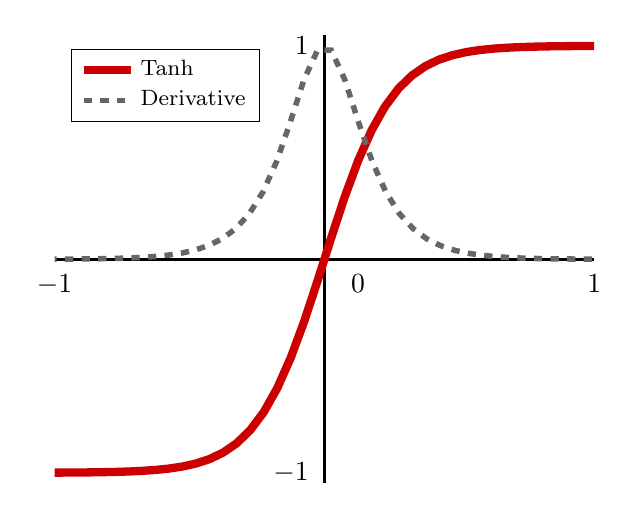
\begin{tikzpicture}
        \begin{axis}[
            axis lines=middle,
            xmax=4,
            xmin=-4,
            ymin=-1.05,
            ymax=1.05,
            xtick={-4,0.5,4},
            ytick={-1,0,1},
            xticklabels={$-1$, $0$, $1$},
            yticklabels={$-1$, $0$,$1$},
            axis line style={-},
            axis line style ={very thick},
            tick style={draw=none},
            label style={font=\scriptsize},
            every axis x label/.style={at={(current axis.right of origin)},anchor=north west},
            every axis y label/.style={at={(current axis.above origin)},anchor=north east},
            legend pos=north west,
            legend style={font=\footnotesize},
            legend cell align={left},
          ]
          \addplot [line width=3pt, domain=-9.9:9.9, samples=100, myred] {(exp(x) - exp(-x))/(exp(x) + exp(-x))};
          \addplot [line width=2pt, dashed, domain=-10:10, samples=100, gray!80!black] {{(1 - tanh(x)^2)/(1 + tanh(x)^2)}};
          \addlegendentry{Tanh}
          \addlegendentry{Derivative}
        \end{axis}
      \end{tikzpicture}
    \end{minipage}
    \begin{minipage}{0.35\textwidth}
      {\begin{center}
          \Large{\textbf{\textcolor{myred}{Hyperbolic Tangent}}}\end{center}}
      {\Large
        \begin{equation*}
          \textcolor{myred}{\tanh{z} = \frac{e^{z}-e^{-z}}{e^{z}+e^{-z}}}
        \end{equation*}
      }
    \end{minipage}
    \begin{minipage}{0.15\textwidth}
      \
    \end{minipage}
  }
\end{figure}
\end{document}